\documentclass[a4paper, 11pt]{article}
\usepackage{longtable}
% LaTeX2e korrigieren.
\usepackage{fixltx2e}
% deutsche Spracheinstellungen
\usepackage{polyglossia}
\setmainlanguage{german}
\usepackage{diagbox}
\usepackage{fullpage}
% unverzichtbare Mathe-Befehle
\usepackage{amsmath}
% viele Mathe-Symbole
\usepackage{amssymb}
% Erweiterungen für amsmath
\usepackage{mathtools}

% Fonteinstellungen
\usepackage{fontspec}
\defaultfontfeatures{Ligatures=TeX}

\usepackage[
  math-style=ISO,    % \
  bold-style=ISO,    % |
  sans-style=italic, % | ISO-Standard folgen
  nabla=upright,     % |
  partial=upright,   % /
]{unicode-math}

\setmathfont{Latin Modern Math}
\setmathfont[range={\mathscr, \mathbfscr}]{XITS Math}
\setmathfont[range=\coloneq]{XITS Math}
\setmathfont[range=\propto]{XITS Math}
% make bar horizontal, use \hslash for slashed h
\let\hbar\relax
\DeclareMathSymbol{\hbar}{\mathord}{AMSb}{"7E}
\DeclareMathSymbol{ℏ}{\mathord}{AMSb}{"7E}

% richtige Anführungszeichen
\usepackage[autostyle]{csquotes}

% Zahlen und Einheiten
\usepackage[
  locale=DE,                   % deutsche Einstellungen
  separate-uncertainty=true,   % Immer Fehler mit \pm
  per-mode=symbol-or-fraction, % m/s im Text, sonst Brüche
]{siunitx}

% chemische Formeln
\usepackage[version=3]{mhchem}

% schöne Brüche im Text
\usepackage{xfrac}

% Floats innerhalb einer Section halten
\usepackage[section, below]{placeins}
% Captions schöner machen.
\usepackage[
  labelfont=bf,        % Tabelle x: Abbildung y: ist jetzt fett
  font=small,          % Schrift etwas kleiner als Dokument
  width=0.9\textwidth, % maximale Breite einer Caption schmaler
]{caption}
% subfigure, subtable, subref
\usepackage{subcaption}
%\usepackage{subfigure}

% Grafiken können eingebunden werden
\usepackage{graphicx}
% größere Variation von Dateinamen möglich
\usepackage{grffile}

% Standardplatzierung für Floats einstellen
\usepackage{float}
\floatplacement{figure}{htbp}
\floatplacement{table}{htbp}

% schöne Tabellen
\usepackage{booktabs}

% Seite drehen für breite Tabellen
\usepackage{pdflscape}

\usepackage{icomma}

% Mars und Venus
\usepackage{marvosym}

% Hyperlinks im Dokument
\usepackage[
  unicode,
  pdfusetitle,    % Titel, Autoren und Datum als PDF-Attribute
  pdfcreator={},  % PDF-Attribute säubern
  pdfproducer={}, % "
]{hyperref}
% erweiterte Bookmarks im PDF
\usepackage{bookmark}

% Trennung von Wörtern mit Strichen
\usepackage[shortcuts]{extdash}

\usepackage[ddmmyyyy]{datetime}
\renewcommand{\dateseparator}{.}
\usepackage[backend=biber]{biblatex}
\addbibresource../lit.bib}

\newcommand\OverfullCenter[1]{\noindent\makebox[\linewidth]{#1}}
\begin{document}
\noindent
\centerline{\small{\textsc{Technische Universität Dortmund}}} \\
\large\textbf{Übungsblatt 04} \hfill \footnotesize\textbf{Sebastian Bange, Alexander Harnisch, Alexander Knodel} \\
\normalsize Computational Physics \hfill \today \\
Prof. Dr. Jan Kierfeld \hfill Abgabefrist: 13.05.2016\\
\noindent\makebox[\linewidth]{\rule{\textwidth}{0.4pt}}
\section*{Aufgabe 1 - Das Doppelpendel}
In Aufgabe 1 wird ein Doppelpendel mit den zwei Massen $m_1$ und $m_2$ an den Stäben der Länge $L_1$, bzw. $L_2$ betrachtet, wie in Abb. \ref{fig:pendel} skizziert.
\begin{figure}
	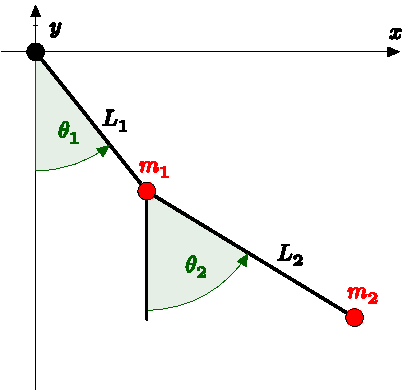
\includegraphics{./blatt.pdf}
	\caption{Doppelpendel aus zwei Massen $m_1$ und $m_2$ an den Stäben der Länge $L_1$, bzw. $L_2$.}
	\label{fig:pendel}
\end{figure}
\\Für die reduzierte Masse $\mu$ gilt mit $m_1 = m_2 = m$:
\begin{equation}
\mu = \frac{m_2}{m_1 + m_2} = \frac{1}{2}
\label{eq:redMasse}
\end{equation}
Die Bewegungsgleichungen für die Winkel $\Theta_i$ ergeben sich zu
\begin{equation}
	\begin{split}
		&\ddot{\Theta_1} = \frac{1}{1-\mu \cos^2(\Theta_2-\Theta_1)} \left[ \mu\,g_1\,\sin(\Theta_2)\,\cos(\Theta_2-\Theta_1)\,\, + \,\, \mu\,\dot{\Theta_1^2}\,\sin(\Theta_2-\Theta_1)\,\cos(\Theta_2-\Theta_1)\right.  \\
		&\left.-g_1\,\sin(\Theta_1)+ \frac{\mu}{\lambda} \dot{\Theta_2^2}\,\sin(\Theta_2-\Theta_1)\right]\\
		&\ddot{\Theta_2} = \frac{1}{1-\mu\,\cos^2(\Theta_2-\Theta_1)}\left[g_2\,\sin(\Theta_1)\cos(\Theta_2-\Theta_1)\,\,-\,\,\mu\,\dot{\Theta_2^2}\,\sin(\Theta_2-\Theta_1)\cos(\Theta_2-\Theta_1)\right. \\
		&\left.-g_2\,\sin(\Theta_2)-\lambda\dot{\Theta_1^2}\,\sin(\Theta_2-\Theta_1)\right]\,. \\
	\end{split}
\label{eq:DGL}
\end{equation}
Weiter gilt $L_1 = L_2 = 1\,\mathup{m}$ und folgende Abkürzungen
\begin{equation*}
	\begin{split}
		 \lambda &:= \frac{L_1}{L_2} = 1 \\
		 g_i &:= \frac{g}{L_i} = 9.81 \frac{1}{\mathup{s}^2} = g \,.
	\end{split}
\end{equation*}
\subsection*{Aufgabenteil a}
Für das System soll die kinetische $T_i$ und potentielle Energie $U_i$ als Funktion der Winkel $\Theta$ und Winkelgeschwindigkeiten $\dot{\Theta}$ aufgestellt werden.\\
Aus den trigonometrischen Winkelbeziehungen und der Überlegung, dass die $x_2$- und $y_2$-Bewegung von der $x_1$- und $y_1$-Bewegung abhängen, folgen

\begin{equation*}
	\begin{split}
		x_1 &= L_1\,\sin(\Theta_1) \\
		y_1 &= L_1\,\cos(\Theta_1) \\
		x_2 &= x_1\,\,+\,\,L_2\,\sin(\Theta_2)\\
		y_2 &= y_1\,\,+\,\,L_2\,\cos(\Theta_2)\\
	\end{split}	
\end{equation*}

Damit können nun die Energiebeiträge aufgestellt werden. Es muss beachtet werden, dass die potentielle Energie am Punkt 1 beide Massen enthält und (durch das Koordinatensystem) negativ ist. Durch die Bewegung des Stabes $L_1$ enthält die kinetische Energie $T_2$ die Bewegung in $x$- und $y$-Richtung

\begin{equation}
	 \begin{split}
 		T_1 &= \frac{m_1}{2}\, L_1^2\, \dot{\Theta_1}^2 \\
 		U_1 &= -\,(m_1+m_2)\,g\,L_1\,\cos(\Theta_1) \\
 		T_2 &= \frac{m_2}{2} \left( \dot{x_2}^2 + \dot{y_2}^2 \right) \\
 			&= \frac{m_2}{2} \left( \dot{\Theta_1}^2\,L_1^2\,\,+\,\,\Theta_2^2\,L_2^2\,\,+\,\,2\,\dot{\Theta_1}\dot{\Theta_2}\,L_1\,L_2\,\cos(\Theta_1-\Theta_2)\right)\\
 		U_2 &= -m_2\,g\,L_2\,\cos(\Theta_2) \,. \\
	 \end{split}
	 \label{eq:Energiebetraege}
\end{equation}

\subsection*{Aufgabenteil b}
Mit den Kleinwinkelnäherungen $\sin(\alpha) \approx \alpha, \cos(\alpha) \approx 1, \cos^2(\alpha) \approx 1$, sowie der Vernachlässigung der $\dot{\Theta_i}^2$-Terme ergibt sich mit Gl. \eqref{eq:redMasse} in Gl. \eqref{eq:DGL}
\begin{equation}
	\begin{split}
		\ddot{\Theta_1} &\approx 2 \left(\frac{1}{2}\,g\,\Theta_2\,\,-\,\,g\,\Theta_1\right) \\
						&= g\,(\Theta_2\,\,-\,\,2\,\Theta_1) := \dot{\Theta_1}\qquad(\Theta_3 := \dot{\Theta_1}) \\
		\ddot{\Theta_2} &\approx 2 \left(g\,\Theta_1\,\,-\,\,g\,\Theta_2\right) := \dot{\Theta_4} \qquad(\Theta_4 := \dot{\Theta_2}) \\
						&= 2\,g\,(\Theta_1\,\,-\,\,\Theta_2) \,. \\
	\end{split}
	\label{eq:DGLTheta}
\end{equation}

Diese beiden DGLs können nun in die Matrixschreibweise überführt werden:
\begin{equation*}
	\begin{split}
		\begin{pmatrix}
			\ddot{\Theta_1} \\
			\ddot{\Theta_2} \\
		\end{pmatrix}
		= g\,
		\begin{pmatrix}
			-2 & 1 \\
			2 & -2 \\
		\end{pmatrix}
		\begin{pmatrix}
			\Theta_1 \\
			\Theta_2 \\
		\end{pmatrix} \,.
	\end{split}
\end{equation*}
Daraus ergeben sich über das charakteristische Polynom die Eigenwerte
\begin{equation*}
 \lambda_{\pm} = -2 \pm \sqrt{2}
\end{equation*}
und die Eigenvektoren (mit zugehöriger Matrix $T$ und inverser Matrix $T^{-1}$)
\begin{equation*}
	\begin{split}
		v_+ &=
		\begin{pmatrix}
			\frac{1}{\sqrt{2}} \\
			1 \\
		\end{pmatrix}
		\qquad
		v_- =
		\begin{pmatrix}
			\frac{-1}{\sqrt{2}} \\
			1 \\
		\end{pmatrix} \\
		\Rightarrow T &=
		\begin{pmatrix}
				\frac{1}{\sqrt{2}} & -\frac{1}{\sqrt{2}} \\
				1 & 1 \\
		\end{pmatrix},\,
		T^{-1} = \frac{1}{2}
		\begin{pmatrix}
				\sqrt{2} & 1 \\
				-\sqrt{2} & 1 \\
		\end{pmatrix}\, . \\
	\end{split}
\end{equation*}
Damit kann nun entkoppelt werden:\\
\begin{equation*}
	\begin{split}
		\vec{\Theta} &:= T \tilde{\Theta} \\
		\Rightarrow \ddot{\Theta} &= T \ddot{\tilde{\Theta}} = A\,T\,\tilde{\theta} \\
		\Rightarrow \ddot{\tilde{\Theta}} &= \underbrace{T^{-1} A T}_{:=L} \tilde{\Theta} \qquad L =\frac{\Theta}{2}
		\begin{pmatrix}
			-4+\sqrt{2} & 0 \\
			0 & -4-\sqrt{2} \,. \\		
		\end{pmatrix}
	\end{split}
\end{equation*}
Damit:
\begin{equation*}
	\begin{split}
		\tilde{\Theta_1} &= c_{11}\,\cos(\omega_1\,t)+c_{12}\,\sin(\omega_1\,t) \qquad w_1^2 = (4-\sqrt{2})\frac{7}{2} \\
		\tilde{\Theta_2} &= c_{21}\,\cos(\omega_2\,t)+c_{22}\,\sin(\omega_2\,t) \qquad w_2^2 = (4+\sqrt{2})\frac{7}{2} \, . \\
	\end{split}
\end{equation*}
In der Rücktransformation ergibt sich:
\begin{equation*}
	\begin{split}
		\Theta &= T \tilde{\Theta} \\
		\Rightarrow \Theta_1 &= \frac{1}{\sqrt{2}} \tilde{\Theta_1} - \frac{1}{\sqrt{2}} \tilde{\Theta_2} = A\,\cos(\omega_1\,t)+B\sin(\omega_1\,t)+C\,\cos(\omega_2\,t)+D\sin(\omega_2\,t) \\
		\Theta_2 &= \tilde{\Theta_1} + \tilde{\Theta_2} = \sqrt{2}\,\left(A\,\cos(\omega_1\,t)+B\sin(\omega_1\,t)-C\,\cos(\omega_2\,t)-D\sin(\omega_2\,t)\right)\,.\\
	\end{split}
\end{equation*}
Die Anfangsbedingungen lauten
\begin{equation*}
	\Theta_{1/2}(0) = \Theta_0^{(1/2)}, \qquad \dot{\Theta}_{1/2}(0) = \dot{\Theta}^{1/2}_0 \,.
\end{equation*}
Aus den vier Gleichungen ergibt sich nach Lösen des LGS:
\begin{equation*}
	\begin{split}
		A &= \frac{\Theta_0^1}{2} + \frac{\Theta_0^2}{2\,\sqrt{2}} \\
		B &= \frac{\dot{\Theta}_0^1}{2\,\omega_1} + \frac{\dot{\Theta}_0^2}{2\,\sqrt{2}\,\omega_1} \\
		C &= \frac{\Theta_0^1}{2} - \frac{\Theta_0^2}{2\,\sqrt{2}} \\
		D &= \frac{\dot{\Theta}_0^1}{2\,\omega_2} - \frac{\dot{\Theta}_0^2}{2\,\sqrt{2}\,\omega_2} \\
	\end{split}
\end{equation*}
Mit \ref{eq:DGLTheta} folgt
\begin{equation*}
	\dot{\vec{\Theta}} = 
	\begin{pmatrix}
		0 & 0 & 1 & 0 \\
		0 & 0 & 0 & 1 \\
		-2\,g & g & 0 & 0 \\
		2\,g & -2\,g & 0 & 0 \\
	\end{pmatrix}
	\vec{\Theta} \stackrel{\text{exp-Ansatz}}{=} \lambda\, \vec{\Theta}
\end{equation*} 

\subsection*{Aufgabenteil c}
Mit den Annahmen aus Aufgabenteil a folgt:
\begin{equation*}
  \begin{split}
  	\rightarrow \overbrace{\dot{\Theta_1}}^{y'(t)} &= \overbrace{\Theta_3}^{f(y)} \stackrel{\text{Code}}{=} dy[0] = y[2]\\
  	\dot{\Theta_2} &= \Theta_4 \stackrel{\text{Code}}{=} dy[1] = y[3] \\
  	\dot{\Theta_3} &= \frac{1}{1-0.5\,\cos^2(\Theta_2-\Theta_1)} \left[ 0.5\,g\,\sin(\Theta_2)\,\cos(\Theta_2-\Theta_1)\,\, + \,\, 0.5\,\dot{\Theta_1^2}\,\sin(\Theta_2-\Theta_1)\,\cos(\Theta_2-\Theta_1)\right.  \\
  	&\left.-g\,\sin(\Theta_1)+ 0.5\, \dot{\Theta_2^2}\,\sin(\Theta_2-\Theta_1)\right] \qquad \stackrel{\text{Code}}{=}  dy[2]\\
  	\dot{\Theta_4} &= \frac{1}{1-0.5\,\cos^2(\Theta_2-\Theta_1)}\left[g\,\sin(\Theta_1)\cos(\Theta_2-\Theta_1)\,\,-\,\,0.5\,\dot{\Theta_2^2}\,\sin(\Theta_2-\Theta_1)\cos(\Theta_2-\Theta_1)\right. \\
		&\left.-g\,\sin(\Theta_2)-0.5\,\dot{\Theta_1^2}\,\sin(\Theta_2-\Theta_1)\right]\qquad \stackrel{\text{Code}}{=}  dy[3]\\\,. \\
  \end{split}
\end{equation*}
Alle $\Theta_i$ und ihre Ableitungen wurden in ein Array geschrieben. Dabei ist $\Theta_1 = y[0]$,$\Theta_2 = y[1]$ usw. Die Masse wurde (wie schon zuvor) auf 1 gesetzt. Sodann werden die Energiebeträge nach \eqref{eq:Energiebetraege} bestimmt. Es wird in kartesische Koordinaten transformiert:
\begin{equation}
 	\begin{split}
 		x_1 &= \sin(\Theta_1) \\
 		y_1 &= \cos(\Theta_1) \\
 		x_2 &= \sin(\Theta_1)+\sin(\Theta_2) \\
 		y_2 &= \cos(\Theta_1)+\cos(\Theta_2) \\ 		
 	\end{split}
 	\label{eq:kartKords}
\end{equation}
Wir haben die $\textsc{swing}$-Methode aufgeteilt, einmal mit Intervall als zweiten Parameter, der dann unter Beachtung des Zaunpfahlproblems in die Stützstellenanzahl gecastet wird. Das Runge-Kutter-Verfahren wird dann für einen Zeitpunkt $t$>0 nach Kürzen des $y$-Arrays außerhalb der Range [$y$, $y+N$) durchgeführt. Analog haben wir das für $t=0$ implementiert. \footnote{Natürlich dann ohne Kürzen. Streng genommen müsste man hier auf $t=0$ prüfen, aber $t<0$ sollte sowieso nie erreicht werden. Weder mathematisch noch physikalisch.}
In der Methode \enquote{$\textsc{save}$} werden alle Daten in entsprechende .dat-files geschrieben. Die grundsätzliche Prozedur ist also immer \enquote{Reset - Initialisieren mit geg. AB. - Pendeln - Speichern}. Die Daten finden sich in den Dateien \enquote{testp1.dat} (positiver Wurzelfall) und \enquote{testp2.dat} (negativer Wurzelfall). Im Terminale \enquote{make} eingeben, um alles generieren zu lassen.
Es folgen die Plots für $Theta_i$ (und ihre Geschwindigkeiten), sowie die Energien (und -beträge). Dabei erkennt man leichte Inkonsistenzen bei der Energieerhaltung, die wir auf Rundungsfehler zurückführen. Die Differenzen betragen dabei $\Delta E_1 = -0.000799999999998$, bzw. $\Delta E_2 = -9.99999999998e-05$ (vgl. out.txt). Es werden  für Schwingungen verschiedener Amplitude und Breite angeregt. Während es im pos. Wurzelfall zu einer Verschiebung bei $\Theta_2$ kommt, ist bei der negativen Wurzel eine deutlich schwächere, breitere Schwingung zu erkennen. Insgesamt sind die Amplituden bei $\Theta_0$ und $\Theta_1$ ähnlich, aber die Breite im Minusfall deutlich geringer. Bei $\Theta_3$ zeigt sich eine deutlich niedrigere Amplitude bei kleinerer Breite. Alle Schwingungen sind harmonisch.
\begin{landscape}
	\begin{figure}
		\OverfullCenter{\includegraphics[width=\textwidth]{../A1/testp1_zeitachse.pdf}}
		\caption{Graphische Darstellung der Ergebnisse von Aufgabe 1 (pos. Wurzel) (Zeitachse).}
		\label{fig:OsziA11}
	\end{figure}
\end{landscape} 

\begin{landscape}
	\begin{figure}
		\OverfullCenter{\includegraphics[width=\textwidth]{../A1/testp2_zeitachse.pdf}}
		\caption{Graphische Darstellung der Ergebnisse von Aufgabe 1 (neg. Wurzel) (Zeitachse).}
		\label{fig:OsziA12}
	\end{figure}
\end{landscape} 

\subsection*{Aufgabenteil d} %Missing

\section*{Poincar\'{e} Schnitt}
\subsection*{Aufgabenteil a}
Unter der Annahme, dass die Geschwindigkeiten auf dem Zettel im unteren mittleren Block für den chaotischen Fall gelten, haben wir wie in Graphik \ref{fig:OsziC1} zu erkennende Phasenraumbilder geplottet. In der $\textsf{Dpendulum.cpp}$ haben wir die Berechnung der Energien rausgeworfen, da nicht explizit gefragt.

\begin{landscape}
	\begin{figure}
		\OverfullCenter{\includegraphics[width=\textwidth]{../A2/teilc.pdf}}
		\caption{Graphische Darstellung der Ergebnisse von Aufgabe 2: Phasenraumbilder für E=3$\,$J,10$\,$J,20$\,$J .}
		\label{fig:OsziC1}
	\end{figure}
\end{landscape} 
\subsection*{Aufgabenteil b}
Die Störung haben wir in der Größenordnung $O(10^{-2})$ implementiert. %Abstand wo?
\begin{landscape}
	\begin{figure}
		\OverfullCenter{\includegraphics[width=\textwidth]{../A2/gestLoesung.pdf}}
		\caption{Graphische Darstellung der Ergebnisse von Aufgabe 2b: Abstände der beiden Trajektorien zur ungestörten Lösung für beide AB.}
		\label{fig:OsziC1}
	\end{figure}
\end{landscape} 
 
\subsection*{Aufgabenteil c}
In der $\textsf{Dpendulum.cpp}$ haben wir den Nulldurchgang dahingehend überprüft, dass wir eine Gerade durch den Durchgang legen und die Punkte vor und hinter dem Nulldurchgang multipliziert ein negatives Vorzeichen besitzen müssen. Über die Ableitung von $x_2$ aus \ref{eq:kartKords} erhält man die zweite Massenbewegung. %x pukt = v und so
Zur Generierung der AB unter konstanter Energie haben wir zufällige Startwerte generiert, mit welchen die Energieerhaltung $\textsc{Etest}$ getestet wird. 
\begin{landscape}
	\begin{figure}
		\OverfullCenter{\includegraphics[width=\textwidth]{../A2/poincare.pdf}}
		\caption{Graphische Darstellung der Ergebnisse von Aufgabe 2c: Poincar\'{e}-Schnitte für E=3$\,$J,10$\,$J,20$\,$J .}
		\label{fig:OsziC1}
	\end{figure}
\end{landscape} 

%\printbibliography
\end{document}
